%Mosfets seul

%transfo avec resistance au secondaire

%2 mosfets avec comparateur

\subsection{Stratégies de balancement}
\paragraph*{}
Les différents modules qui compose la batterie n'on pas exactement la même capacité et la même résistance en série. Ces différences font en sorte que les modules n'atteindront pas un état de charge complet en même temps. Pour égaliser les tensions, le courant de recharge des modules qui ont atteint le voltage maximum peut être dissipé ou envoyé vers les modules qui on un état de charge inférieur. 

\subsubsection*{Balancement dissipatif au voltage maximum des modules ("Top balancing")}
\paragraph*{}
Le balancement dissipatif à l'avantage d'être plus compacte, plus facile à concevoir et moins dispendieux. Le courant de recharge doit cependant pouvoir être réduit pour ne pas être plus haut que le courant de balancement. Cette technique ne permet pas de balancer avec de grand courant puisque la chaleur dégagé par la résistance et le MOSFET dégagerait trop de chaleur, ce qui peut causer une erreur de température élevé. La sensibilité du MOSFET et sa défaillance en court-circuit font en sorte que cette méthode n'est pas très robuste. Au MOSFET en court-circuit ne déclenche aucune erreur et il peut être long avant de détecter qu'un module se vide plus rapidement que les autres. Cette erreur à le potentiel de briser la batterie dans le cas ou aucune action externe n'est prise et que le module atteint une tension en dessous du seuil minimum.

\paragraph*{}
Pour remédier à ce problème, un MOSFET contrôlé par un comparateur est mis en série avec le circuit de balancement. Cette redondance permet de couper le circuit dans lorsque la tension du module n'est pas dans la plage où il peut être balancé. Cette protection est indépendante et matériel, elle est tout aussi efficace dans le cas où le MOSFET contrôlé par le PWM est en court-circuit ou si l'erreur provient du microcontrôleur qui envoi un PWM alors qu'il ne devrait pas.

\begin{figure}[H]
	\begin{minipage}{0.5\textwidth}
		\centering
		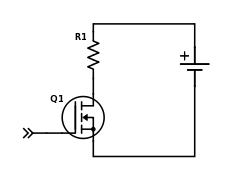
\includegraphics[scale=0.9]{Images/Dissipative_balancing.png}
		\caption{Schéma fonctionnel du balancement dissipatif}
		\label{fig:bal_dis}
	\end{minipage}
	\hfill
	\begin{minipage}{0.45\textwidth}
		\centering
		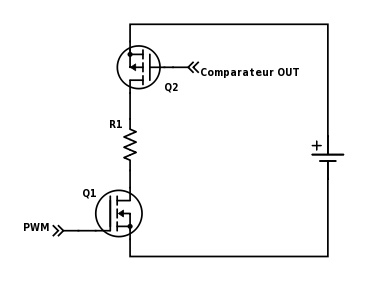
\includegraphics[scale=0.6]{Images/Dissipative_bal_comp.png}
		\caption{Schéma fonctionnel du balancement dissipatif avec redondance}
		\label{fig:bal_dis_comp}
	\end{minipage}	
\end{figure}

\subsubsection*{Balancement actif}
\paragraph*{}




